\newpage

\section{Methodology}

Due to the Heliotron J experimental campaigns nature, the parameters are continuously being changed, resulting in different heating behaviors and instrumentation being off for some shots. The unique configuration of the device ($L=1, M=4$ helical-axis) allows for high operational flexibility, enabling independent control over the rotational transform, magnetic well depth, and bumpy field components. This flexibility, while beneficial for exploring diverse confinement regimes, fundamentally alters the energetic particle confinement and MHD stability landscape from shot to shot if changed. 

Consequently, the shot selection required a rigorous filtering process to ensure consistent magnetic topologies and heating schemes were compared. These shots are available at the link presented in the annex \ref{annex:data} Also, a visually diagnosis for the Mirnov and frequency behavior was made, ensuring that the analysis was being executed on well behaved data that can later be extrapolated to more complex experimental results. This visual screening was critical to reject discharges where the magnetic signals were severely corrupted by operational artifacts, such as power supply switching noise, external RF pickup, or atypical plasma termination events. On the figure \ref{fig:methodology_pipeline}, the methodology pipeline is presented, being extended on the posterior subsections. The GitHub repository with the python codes used in order to execute this methodology is available at the appendix \ref{appendix:github}.

\begin{figure}[H]
  \centering
  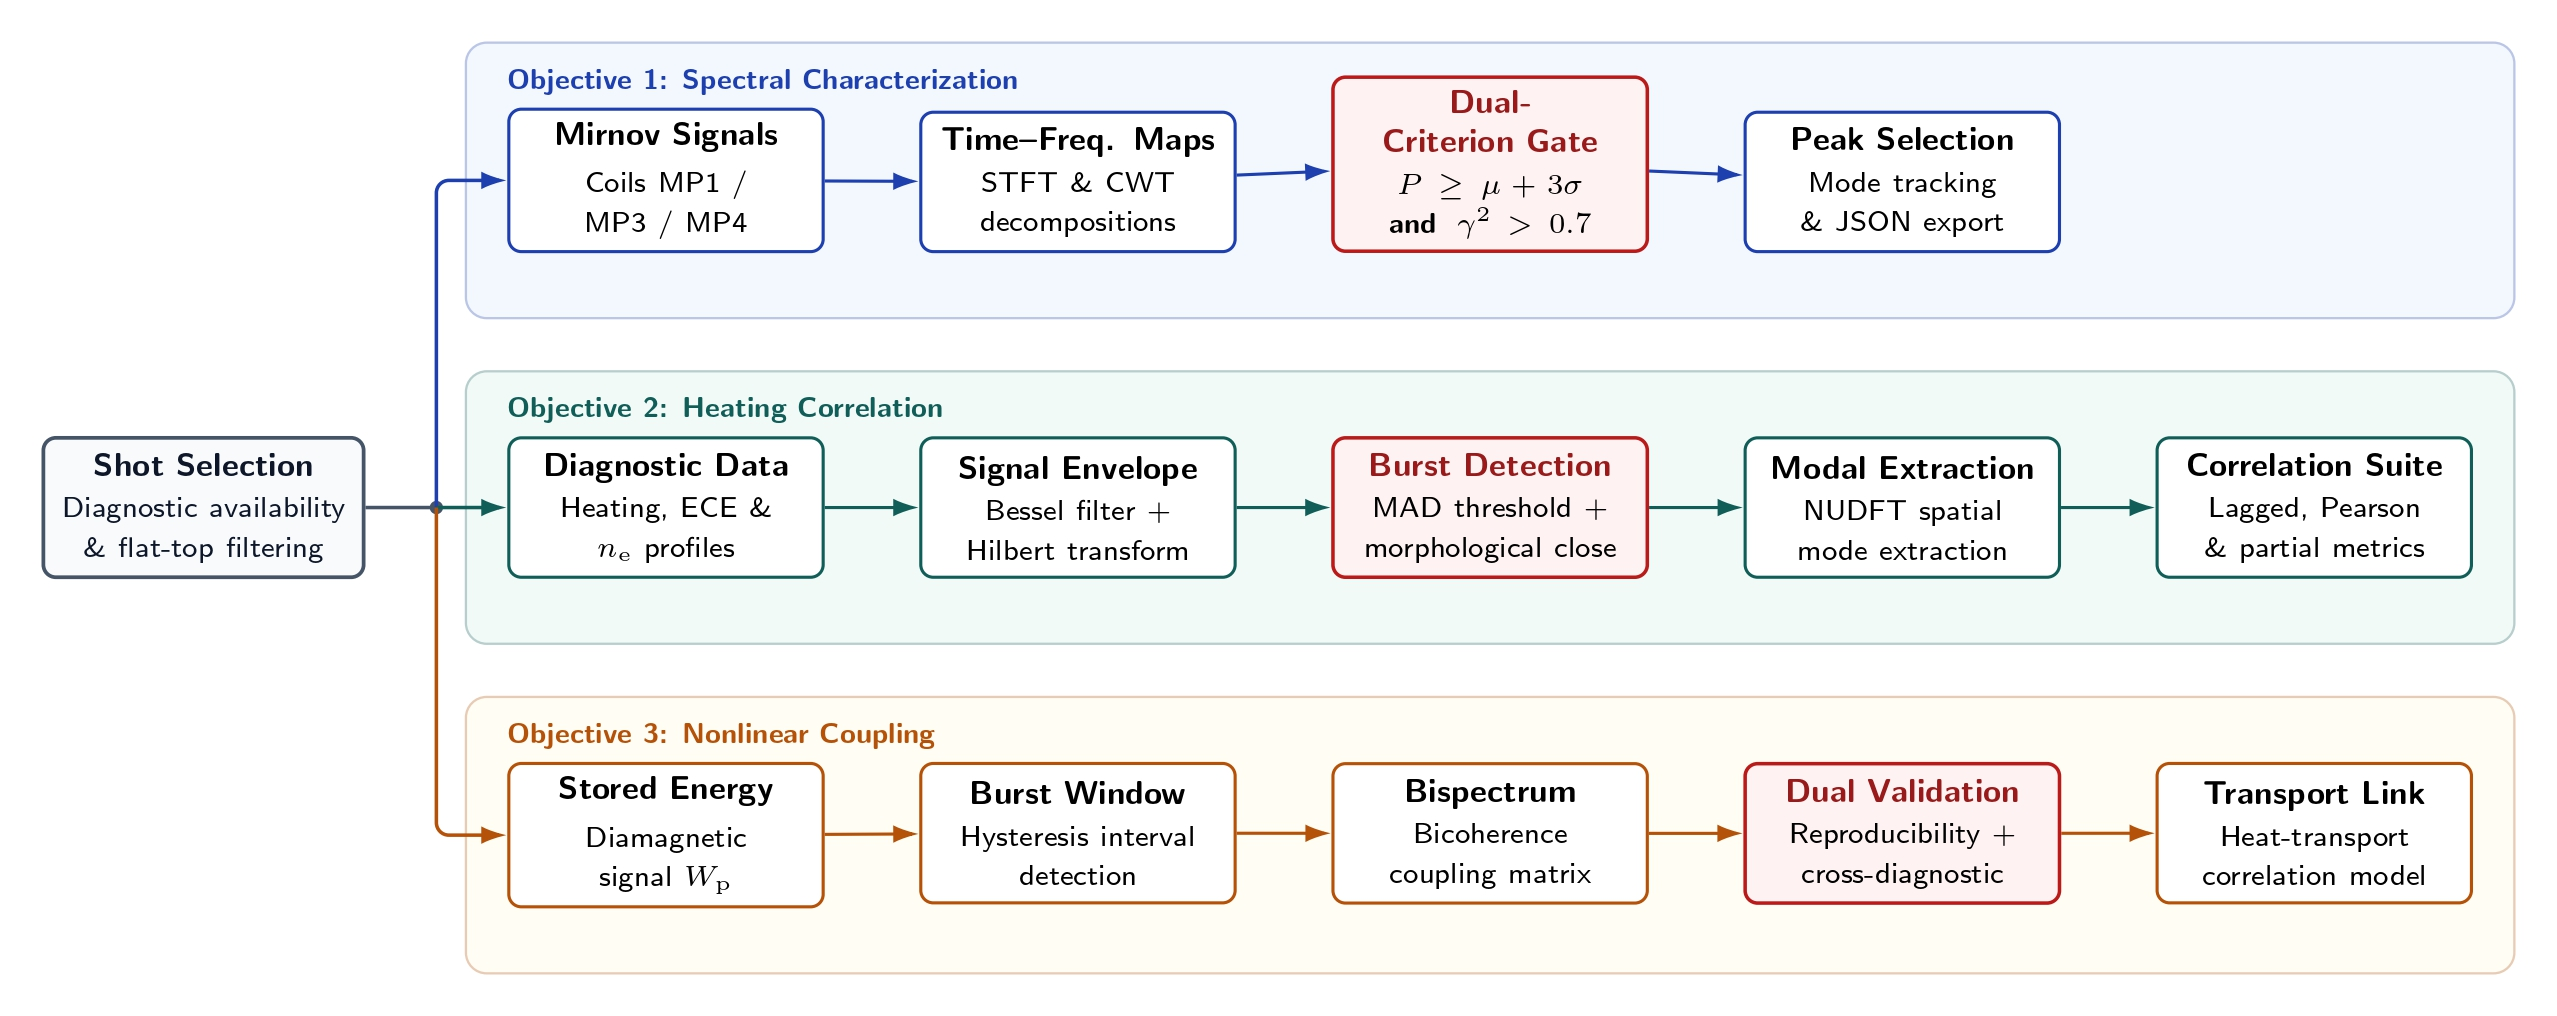
\includegraphics[width=\textwidth]{Images/pipeline.jpg}
  \caption[Methodology pipeline]{Methodology pipeline. Source: Own elaboration.}
  \label{fig:methodology_pipeline}
\end{figure}
\newpage


\subsection{First Specific Objective}
This objective centers in the characterizing of the spectral properties and temporal evolution of  the MHD oscillations in the Heliotron J device \cite{nagasaki2020heliotron, Yamamoto_2020}. For this matter, a Python pipeline applies a rigorous dual-criterion validation to isolate physical modes from background noise that will be expanded next.

\subsubsection{Data Acquisition and Preprocessing}
Magnetic fluctuation data from Mirnov coils MP1, MP3, and MP4 were imported via the \texttt{turnelib} library from the jpack library, available in the annex \ref{annex:library}. MP1 served as the spectral reference, while MP3 and MP4 provided spatial cross-validation. Channel MP2 was specifically excluded from this configuration due to its non-zero poloidal angle, which would introduce confounding phase artifacts into the purely toroidal mode analysis, compromising the validity of the results \cite{Seo2019TheEO,schittenhelm1997analysis}.

\subsubsection{Time-Frequency Analysis}
Two complementary representations of the MP1 signal captured stationary and transient dynamics:
\begin{itemize}
    \item STFT: A windowed Fast Fourier Transform with the jpack package called \texttt{libana\_signal}, available in the annex \ref{annex:library} using a Hann window generated a Power Spectral Density (PSD) spectrogram presented in the equation \ref{eqn:freq_res} \cite{proakis2021digital}, dynamically scaled for a constant $500~\mathrm{Hz}$ resolution.
    \item CWT: A complex Morlet wavelet ($\omega_0 = 6$) based in equation \ref{eqn:morlet} \cite{boashash2015time, addison2016illustrated} resolved fast transients. Time support scaled to $\pm 5$ standard deviations across 150 frequency bins ($10~\mathrm{kHz}$ to $150~\mathrm{kHz}$).
\end{itemize}



\subsubsection{Dual-Criterion Mode Identification}
For a mode to be a confirmed physical mode, it requires simultaneous statistical and spatial validation:
\begin{itemize}
    \item Statistical Dominance: A baseline $3\sigma$ threshold, as seen in the equation Eq. \ref{eqn:dominance} \cite{Edlund2018} was calibrated using a $0$ to $25~\mathrm{ms}$ pre-plasma window. Smoothed spectral power ($4~\mathrm{ms}$ rolling average) had to continuously exceed this threshold for $\geq 2~\mathrm{ms}$.
    \item Spatial Coherence: Welch's method (100 ensembles) evaluated magnitude-squared coherence ($\gamma^2$), visible in the equation \ref{eqn:coherence} \cite{KraemerFlecken2024, Singh2024} between MP1-MP3, MP1-MP4, and MP3-MP4. The convention for valid modes requires $\gamma^2 > 0.7$ on at least one pair.
\end{itemize}


\subsubsection{Peak Selection and Export}
Finally, the prominent peaks ($15~\mathrm{kHz}$ to $100~\mathrm{kHz}$) that passed the criteria were isolated, separating the dominant only against the dominant and coherent. Mode properties, such as frequency, amplitude, active intervals were exported to a .JSON file, alongside visual diagnostic summaries such as a time dependent 3$\sigma$ spectrogram, the Morlet Wavelet Transform time dependency, and the coherence distributions for all the frequencies.

\subsection{Second Specific Objective}
The second objective mission is to evaluate correlations between EPMs and plasma heating (NBI and ECH) using the magnetic fluctuation frequencies \cite{Adulsiriswad_2024, Zhong2024, Zhong2020}, more detail is presented next.

\subsubsection{Signal Conditioning and Active Burst Detection}
Heating, ECE, and density signals were linearly interpolated onto the Mirnov time base. The complete signal-conditioning and dynamic parameter extraction sequence is summarized in the figure \ref{fig:methodology2} and is expanded on the following subsubsections, providing a deeper submersion on the data treatment.

\begin{figure}[H]
  \centering
  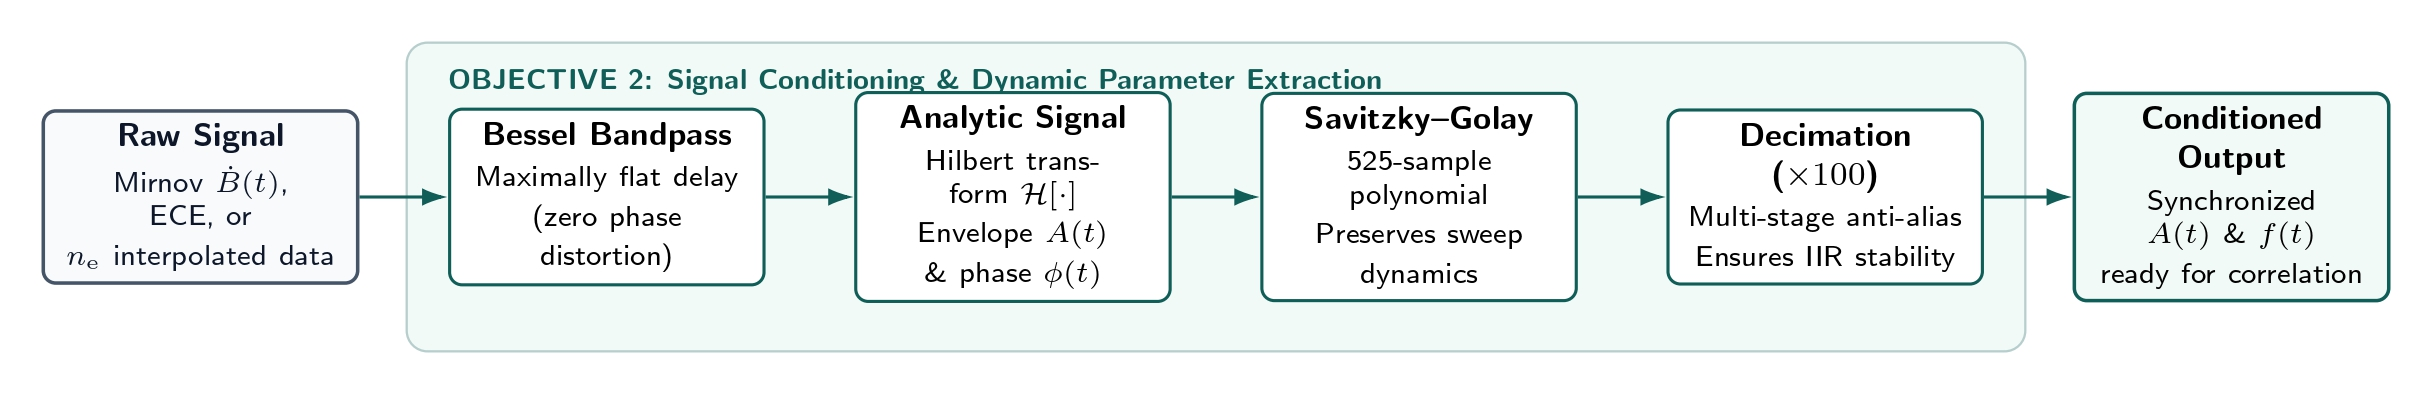
\includegraphics[width=\textwidth]{Images/obj2methodology.jpg}
  \caption[Signal-conditioning and parameter-extraction chain for Objective 2]{Signal-conditioning and parameter-extraction chain for Objective 2. Source: Own elaboration.}
  \label{fig:methodology2}
\end{figure}


Starting with a Bessel bandpass filter and a Hilbert transform that extracted the mode's instantaneous amplitude and phase \cite{zang2019observation, Fabus2021}. Then, to make sure that the physical frequency sweeps are not artificially flattened, the Savitzky-Golay filter utilizes a statically optimized window size of 525 samples, a value confirmed via offline sensitivity sweeps to best preserve the mode's instantaneous frequency dynamics.

Analyses were restricted to a dynamically thresholded active window. This threshold is established using the full-trace median plus $6.0$ times the standard-deviation-equivalent Median Absolute Deviation ($1.4826 \times \mathrm{MAD}$) to accurately represent the heated baseline noise floor. A binary closing morphological operation, bridging gaps up to $3.0~\mathrm{ms}$, is subsequently applied to isolate the single largest contiguous mode-active burst, rejecting noise spikes shorter than $10.0~\mathrm{ms}$. Furthermore, prior to correlation analysis, the envelope and frequency arrays undergo a cascaded anti-aliasing decimation, with a total factor of 100, utilizing iterative intermediate downsampling steps to mathematically maintain low-pass Infinite Impulse Response (IIR) filter stability while respecting the temporal Nyquist limit \cite{boashash2015time, Fabus2021}.

\subsubsection{Modal Structure Extraction}
A non-uniform discrete Fourier transform (NUDFT) across coils PMP1--PMP14 was used in order to extract the poloidal mode number ($m$) from the analyzed mode at this shot (Eq. \ref{eqn:nudft}, \ref{eqn:pol_phase}) \cite{Varela2019}. Voltages were converted to $\mathrm{T}/\mathrm{s}$, and inverted wirings (PMP1--PMP4) were corrected, from the original code provided by the Heliotron J team, and available in the annex \ref{annex:poloidalm}. Search boundaries spanned $m = \pm 6$, automatically expanding to $\pm 20$ if peak-pinned.
Inter-probe coherence was gated by a flat-frequency sub-window algorithm anchored to the Objective 1 active intervals. A sliding $8.0~\mathrm{ms}$ window located the core with the lowest local slope $|\mathrm{d}f/\mathrm{d}t|$, growing within a $50~\%$ tolerance to evaluate coherence strictly over the non-chirping plateau.

\subsubsection{Correlation with Heating Systems}
Mode parameters and heating profiles were synchronized using statistical metrics:

\begin{itemize}
    \item Lagged Cross-Correlation: Scanned $\pm 20.0~\mathrm{ms}$ for amplitude, $\pm 40.0~\mathrm{ms}$ for frequency, and $\pm 50.0~\mathrm{ms}$ for core proxies in order to evaluate hysteresis, as stated in equation \ref{eqn:lagged_corr} \cite{Zhong2020}.
    \item Pearson Correlation: Required $|r| > 0.7$ and $p < 0.05$, adjusting effective sample size ($N_{\mathrm{eff}}$) for serial autocorrelation, like in equations  \ref{eqn:neff} and \ref{eqn:t_stat} \cite{shumway2017time}.
    \item Partial Correlation: Rejected shared-step artifacts (e.g., ECH turn-off), verified via binarization threshold sweeps ($30~\%$ to $70~\%$), this is basd in equation   \ref{eqn:partial_corr} \cite{james2021statistical}.
    \item Correction: Applied Bonferroni and the Benjamini-Hochberg procedure for the False Discovery Rate FDR-BH adjustments, systematically excluding low-power tests ($N_{\mathrm{eff}} < 5$) \cite{dunn1961multiple, Benjamini1995}.

\end{itemize}




\subsubsection{Energetic-Particle Distribution and Alfvén Scaling}
Temporal delays between mode dynamics and core ECE proxies were evaluated against the Spitzer electron-drag timescale ($\tau_s$) presented in equation \ref{eqn:slowing_down} \cite{Salewski2025}. ECE channels were selected by highest zero-lag correlation to ECH power, strictly filtering ADC-saturated channels (e.g., $> 20$ static samples).
Frequency sweeping was validated against Alfvén velocity scaling, displayed in equations \ref{eqn:alfven} and \ref{eqn:shear_alfven} \cite{chen2016introduction, Varela2024} using a $1.25~\mathrm{T}$ field and median-filtered ($n=5$) electron density, interpolating over transient ECH glitches. Since $r$ is mathematically invariant to the positive-scalar normalization constant these windows produce, invariance was verified across calibration sub-windows spanning $150.0~\mathrm{ms}$ to $285.0~\mathrm{ms}$, with the reported result computed on the $250.0~\mathrm{ms}$--$270.0~\mathrm{ms}$ window.

\subsection{Third Specific Objective}
This final specific objective characterizes the low-frequency H-mode fluctuations by mapping nonlinear coupling events associated with edge turbulence and heat transport \cite{Kin2025, Miyashita2025}, as presented next.

\subsubsection{H-mode Burst-Window Detection and Sub-Window Refinement}
The stored energy signal ($W_p$) partitioned the discharge into burst ($k_{\mathrm{on}} = 3.0$) and back-transition ($k_{\mathrm{off}} = 1.5$) windows \cite{Kin2025}, requiring a $10~\mathrm{ms}$ minimum duration. To define the quiescent and control windows, the algorithm searched outward from the burst edges in $2.0~\mathrm{ms}$ increments, starting beyond a $5.0~\mathrm{ms}$ boundary margin, to find the nearest genuinely flat, sub-threshold $25.0~\mathrm{ms}$ segments. The acceptable flatness criteria was strictly self-calibrated to the discharge's empirical background, requiring the segment's variance score to fall below $1.5$ times the median ($50^{\mathrm{th}}$ percentile) spread of equivalently sized background windows.
Bicoherence limits were tightened via an $8.0~\mathrm{ms}$ flat-frequency sub-window applied to MP1 (Bessel-filtered $5.0\text{--}100.0~\mathrm{kHz}$), grown within a $50~\%$ tolerance until chirping limits forced iteration to meet FFT sample floors ($N_{\mathrm{fft}} = 1024$, $N_{\mathrm{ensemble}} = 30$).

\subsubsection{Bicoherence Calculation and Peak Identification}
Squared auto-bicoherence $b^2(f_1, f_2)$ evaluated Sum and Difference interactions, presented in equations \ref{eqn:bispectrum}, \ref{eqn:bicoherence}, \ref{eqn:sum_domain} and \ref{eqn:diff_domain} \cite{Hou2019, Fujisawa2021}. Significance required surpassing $b^2 > 0.5$ \cite{Singh2024} and a $95~\%$ statistical noise threshold ($b^2_{95} = -\ln(0.05)/N_{\mathrm{ensemble}}$) stated in equation \ref{eqn:b2_stat} \cite{Hou2019, Fujisawa2021}.
Searches were restricted below $100.0~\mathrm{kHz}$ with a $5.0~\mathrm{kHz}$ minimum floor. Peaks identified via a 2D maximum filter ($5.0~\mathrm{kHz}$) were subjected to boundary ($10.0~\mathrm{kHz}$) and inner-core stability checks. Triads were confirmed within $1.5$ bins of genuine PSD peaks. An RMS amplitude check flagged array channels deviating $5\times$ from the median.

\subsubsection{Validation Criteria}
Statistical superiority of burst-window bicoherence was verified via Kruskal-Wallis and Mann-Whitney U tests ($\alpha = 0.025$) \cite{shumway2017time, james2021statistical}. Candidate couplings required strict double-validation:

\begin{itemize}
    \item Reproducibility: Leading peaks ($b^2 > 0.5$) must replicate within $\pm 10.0~\mathrm{kHz}$ in an independent validation discharge.
    \item Cross-Diagnostic Consistency: Magnetic signatures must concurrently appear in the divertor Langmuir array (excluding non-physical bias/trigger pins). Tip couplings were gated by a multiple-comparisons check ($p < 0.05$) based on the array's effective independent channels, based in equations  \ref{eqn:meff} and \ref{eqn:p_chance}) \cite{Bishop2023, Afyouni2019}.
\end{itemize}



\subsubsection{Heat Transport Correlation}
Elevated burst-phase bicoherence was ultimately validated against periods of degraded or negative temporal stored energy derivatives ($\langle \mathrm{d}W_p/\mathrm{d}t \rangle$), confirming three-wave coupling mediation of enhanced turbulent transport \cite{Hou2019, Fujisawa2021}.